\documentclass{article}
%%%%%%%%%%%%%%%%%%%%%%%%%%%%%%%%%%%%%%%%%
% Lachaise Assignment
% Structure Specification File
% Version 1.0 (26/6/2018)
%
% This template originates from:
% http://www.LaTeXTemplates.com
%
% Authors:
% Marion Lachaise & François Févotte
% Vel (vel@LaTeXTemplates.com)
%
% License:
% CC BY-NC-SA 3.0 (http://creativecommons.org/licenses/by-nc-sa/3.0/)
% 
%%%%%%%%%%%%%%%%%%%%%%%%%%%%%%%%%%%%%%%%%

%----------------------------------------------------------------------------------------
%	PACKAGES AND OTHER DOCUMENT CONFIGURATIONS
%----------------------------------------------------------------------------------------

\usepackage{amsmath,amsfonts,stmaryrd,amssymb,subcaption} % Math packages

\usepackage{enumerate} % Custom item numbers for enumerations

\usepackage[ruled]{algorithm2e} % Algorithms

\usepackage[framemethod=tikz]{mdframed} % Allows defining custom boxed/framed environments

\usepackage{listings} % File listings, with syntax highlighting
\lstset{
	basicstyle=\ttfamily, % Typeset listings in monospace font
}

%----------------------------------------------------------------------------------------
%	DOCUMENT MARGINS
%----------------------------------------------------------------------------------------

\usepackage{geometry} % Required for adjusting page dimensions and margins

\geometry{
	paper=a4paper, % Paper size, change to letterpaper for US letter size
	top=2cm, % Top margin
	bottom=2.5cm, % Bottom margin
	left=2cm, % Left margin
	right=2cm, % Right margin
	headheight=14pt, % Header height
	footskip=1.5cm, % Space from the bottom margin to the baseline of the footer
	headsep=1.2cm, % Space from the top margin to the baseline of the header
	%showframe, % Uncomment to show how the type block is set on the page
}

%----------------------------------------------------------------------------------------
%	FONTS
%----------------------------------------------------------------------------------------

\usepackage[utf8]{inputenc} % Required for inputting international characters
\usepackage[T1]{fontenc} % Output font encoding for international characters

\usepackage{XCharter} % Use the XCharter fonts

%----------------------------------------------------------------------------------------
%	COMMAND LINE ENVIRONMENT
%----------------------------------------------------------------------------------------

% Usage:
% \begin{commandline}
%	\begin{verbatim}
%		$ ls
%		
%		Applications	Desktop	...
%	\end{verbatim}
% \end{commandline}

\mdfdefinestyle{commandline}{
	leftmargin=10pt,
	rightmargin=10pt,
	innerleftmargin=15pt,
	middlelinecolor=black!50!white,
	middlelinewidth=2pt,
	frametitlerule=false,
	backgroundcolor=black!5!white,
	frametitle={Command Line},
	frametitlefont={\normalfont\sffamily\color{white}\hspace{-1em}},
	frametitlebackgroundcolor=black!50!white,
	nobreak,
}

% Define a custom environment for command-line snapshots
\newenvironment{commandline}{
	\medskip
	\begin{mdframed}[style=commandline]
}{
	\end{mdframed}
	\medskip
}

%----------------------------------------------------------------------------------------
%	FILE CONTENTS ENVIRONMENT
%----------------------------------------------------------------------------------------

% Usage:
% \begin{file}[optional filename, defaults to "File"]
%	File contents, for example, with a listings environment
% \end{file}

\mdfdefinestyle{file}{
	innertopmargin=1.6\baselineskip,
	innerbottommargin=0.8\baselineskip,
	topline=false, bottomline=false,
	leftline=false, rightline=false,
	leftmargin=2cm,
	rightmargin=2cm,
	singleextra={%
		\draw[fill=black!10!white](P)++(0,-1.2em)rectangle(P-|O);
		\node[anchor=north west]
		at(P-|O){\ttfamily\mdfilename};
		%
		\def\l{3em}
		\draw(O-|P)++(-\l,0)--++(\l,\l)--(P)--(P-|O)--(O)--cycle;
		\draw(O-|P)++(-\l,0)--++(0,\l)--++(\l,0);
	},
	nobreak,
}

% Define a custom environment for file contents
\newenvironment{file}[1][File]{ % Set the default filename to "File"
	\medskip
	\newcommand{\mdfilename}{#1}
	\begin{mdframed}[style=file]
}{
	\end{mdframed}
	\medskip
}

%----------------------------------------------------------------------------------------
%	NUMBERED QUESTIONS ENVIRONMENT
%----------------------------------------------------------------------------------------

% Usage:
% \begin{question}[optional title]
%	Question contents
% \end{question}

\mdfdefinestyle{question}{
	innertopmargin=1.2\baselineskip,
	innerbottommargin=0.8\baselineskip,
	roundcorner=5pt,
	nobreak,
	singleextra={%
		\draw(P-|O)node[xshift=1em,anchor=west,fill=white,draw,rounded corners=5pt]{%
		Question \theQuestion\questionTitle};
	},
}

\newcounter{Question} % Stores the current question number that gets iterated with each new question

% Define a custom environment for numbered questions
\newenvironment{question}[1][\unskip]{
	\bigskip
	\stepcounter{Question}
	\newcommand{\questionTitle}{~#1}
	\begin{mdframed}[style=question]
}{
	\end{mdframed}
	\medskip
}

%----------------------------------------------------------------------------------------
%	WARNING TEXT ENVIRONMENT
%----------------------------------------------------------------------------------------

% Usage:
% \begin{warn}[optional title, defaults to "Warning:"]
%	Contents
% \end{warn}

\mdfdefinestyle{warning}{
	topline=false, bottomline=false,
	leftline=false, rightline=false,
	nobreak,
	singleextra={%
		\draw(P-|O)++(-0.5em,0)node(tmp1){};
		\draw(P-|O)++(0.5em,0)node(tmp2){};
		\fill[black,rotate around={45:(P-|O)}](tmp1)rectangle(tmp2);
		\node at(P-|O){\color{white}\scriptsize\bf !};
		\draw[very thick](P-|O)++(0,-1em)--(O);%--(O-|P);
	}
}

% Define a custom environment for warning text
\newenvironment{warn}[1][Warning:]{ % Set the default warning to "Warning:"
	\medskip
	\begin{mdframed}[style=warning]
		\noindent{\textbf{#1}}
}{
	\end{mdframed}
}

%----------------------------------------------------------------------------------------
%	INFORMATION ENVIRONMENT
%----------------------------------------------------------------------------------------

% Usage:
% \begin{info}[optional title, defaults to "Info:"]
% 	contents
% 	\end{info}

\mdfdefinestyle{info}{%
	topline=false, bottomline=false,
	leftline=false, rightline=false,
	nobreak,
	singleextra={%
		\fill[black](P-|O)circle[radius=0.4em];
		\node at(P-|O){\color{white}\scriptsize\bf i};
		\draw[very thick](P-|O)++(0,-0.8em)--(O);%--(O-|P);
	}
}

% Define a custom environment for information
\newenvironment{info}[1][Info:]{ % Set the default title to "Info:"
	\medskip
	\begin{mdframed}[style=info]
		\noindent{\textbf{#1}}
}{
	\end{mdframed}
}
 % Include the file specifying the document structure and custom commands
\setlength\parindent{0pt}

\title{EECS 545: Homework \#2} % Title of the assignment

\author{Mingliang Duanmu\\ \texttt{duanmuml@umich.edu}} % Author name and email address

\date{\today} % University, school and/or department name(s) and a date

\begin{document}

\maketitle % Print the title

\section{Logistic regression}

\subsection*{a}

For each element in $\mathbf{H}$, we have
$$H_{ij} = \frac{\partial^2 E}{\partial w_i \partial w_j}$$
Since $H_{ij} = 0$ when $i \neq j$, we have
$$
\begin{aligned}
H_{jj} = & \frac{\partial^2}{\partial w_j^2}\sum_{i=1}^N -(y^{(i)}\log \sigma(\mathbf{w}^T\mathbf{x}^{(i)}) + (1 - y^{(i)})\log (1 - \sigma(\mathbf{w}^T\mathbf{x}^{(i)}))) \\
= & \frac{\partial}{\partial w_j} \sum_{i=1}^N x_j^{(i)} (\sigma(w_j x_j^{(i)}) - y^{(i)}) \\ 
= & -\sum_{i=1}^N((x_j^{(i)})^2\sigma (w_j x_j^{(i)})(1 - \sigma (w_j x_j^{(i)}))
\end{aligned}
$$
Therefore, we can represent hessian $\mathbf{H}$ as
$$\mathbf{H} = -\mathbf{x}^T\mathbf{S}\mathbf{x}$$
where
$$S_{ii} = \sigma(\mathbf{w}^T\mathbf{x}^{(i)}) (1 - \sigma(\mathbf{w}^T\mathbf{x}^{(i)}))$$
$$S_{ij} = 0 (i \neq j)$$
Therefore,
$$\mathbf{z}^T\mathbf{H}\mathbf{z} = -\mathbf{z}^T\mathbf{x}^T\mathbf{S}\mathbf{x}\mathbf{z} = -\Sigma_i \Sigma_j z_ix_ix_jz_j \sigma(\mathbf{w}^T\mathbf{x}^{(i)}) (1 - \sigma(\mathbf{w}^T\mathbf{x}^{(i)})) = -(\mathbf{x}^T\mathbf{z})^2 p(1-p) \leq 0$$
where $0 \leq p \leq 1$, so the hessian is negative semi-definite and thus $\ell$ is concave and has no local maxima other than the global one.

\subsection*{b}

The update rule implied by Newton's method is
$$\mathbf{w}_{n+1} = \mathbf{w}_n - \mathbf{H}_{\ell(\mathbf{w})}^{-1} \nabla \ell(\mathbf{w})$$
The fitted coefficients are [-1.84922892 -0.62814188  0.85846843].

\newpage

\subsection*{c}

\begin{figure}[htbp]
    \centering
    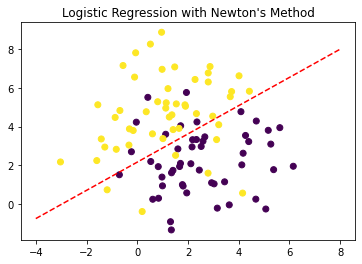
\includegraphics[width=.6\textwidth]{q1.png}
\end{figure}

\section{Softmax Regression via Gradient Ascent}

\subsection*{a}

For $y^{(i)} = k \neq m$, we have
$$
\begin{aligned}
& \nabla_{w_{m}}(\mathbf{I}(y^{(i)}=k)  p(y^{(i)}=k \mid \mathbf{x}^{(i)}, \mathbf{w})) \\
=& \mathbf{I}(y^{(i)}=k)  \nabla_{w_{m}}(\frac{\exp (\mathbf{w}_{k}^{T} \phi(\mathbf{x}^{(i)}))}{1+\sum_{j=1}^{K-1} \exp (\mathbf{w}_{j}^{T} \phi(\mathbf{x}^{(i)}))}) \\
=& \mathbf{I}(y^{(i)}=k)  \phi(\mathbf{x}^{(i)}) (-\frac{\exp (\mathbf{w}_{k}^{T} \phi(\mathbf{x}^{(i)}))}{1+\sum_{j=1}^{K-1} \exp (\mathbf{w}_{j}^{T} \phi(\mathbf{x}^{(i)}))})
\end{aligned}
$$
For $y^{(i)} = k = m$, we have
$$
\begin{aligned}
& \nabla_{w_{m}}(\mathbf{I}(y^{(i)}=k)  p(y^{(i)}=k \mid \mathbf{x}^{(i)}, \mathbf{w})) \\
=& \mathbf{I}(y^{(i)}=k)  \nabla_{w_{m}}(\frac{\exp (\mathbf{w}_{k}^{T} \phi(\mathbf{x}^{(i)}))}{1+\sum_{j=1}^{K-1} \exp (\mathbf{w}_{j}^{T} \phi(\mathbf{x}^{(i)}))}) \\
=& \mathbf{I}(y^{(i)}=k)  \phi(\mathbf{x}^{(i)}) (1-\frac{\exp (\mathbf{w}_{k}^{T} \phi(\mathbf{x}^{(i)}))}{1+\sum_{j=1}^{K-1} \exp (\mathbf{w}_{j}^{T} \phi(\mathbf{x}^{(i)}))})
\end{aligned}
$$
By summing up all the classes, we have
$$
\begin{aligned}
\nabla_{\mathbf{w}_{m}} l(\mathbf{w}) &=\sum_{i=1}^{N} \phi(\mathbf{x}^{(i)}) \sum_{k=1}^{K}(\mathbf{I}(y^{(i)}=k)  p(y^{(i)}=k \mid \mathbf{x}^{(i)}, \mathbf{w})) \\
&=\sum_{i=1}^{N} \phi(\mathbf{x}^{(i)})\left[\mathbf{I}(y^{(i)}=m)-p(y^{(i)}=m \mid \mathbf{x}^{(i)}, \mathbf{w})\right]
\end{aligned}
$$

\subsection*{b}

The accuracy of the softmax regression implementation is 94\%, which is greater than the \texttt{sklearn} logistic regression model.

\section{Gaussian Discriminate Analysis}

\subsection*{a}

According to Bayes Rule,
$$
\begin{aligned}
p(y=1 \mid \mathbf{x} ; \phi, \Sigma, \mu_{0}, \mu_{1}) &=\frac{p(\mathbf{x} \mid y=1) p(y=1)}{p(\mathbf{x} \mid y=0) p(y=0)+p(\mathbf{x} \mid y=1) p(y=1)} \\
& = \frac{1}{1+\frac{p(\mathbf{x} \mid y=0) p(y=0)}{p(\mathbf{x} \mid y=1) p(y=1)}}
\end{aligned}
$$
where
$$
\begin{aligned}
& \frac{p(\mathbf{x} \mid y=0) p(y=0)}{p(\mathbf{x} \mid y=1) p(y=1)} \\ 
= & \exp (-\frac{1}{2}(\mathbf{x}-\mu_{0})^{T} \Sigma^{-1}(\mathbf{x}-\mu_{0})+\frac{1}{2}(\mathbf{x}-\mu_{1})^{T} \Sigma^{-1}(\mathbf{x}-\mu_{1})) \frac{p(y=0)}{p(y=1)} \\
= & \exp (\frac{1}{2}(\mu_{1}^{T} \Sigma^{-1} \mu_{1}-\mu_{0}^{T} \Sigma^{-1} \mu_{0}) + \log \frac{p(y=0)}{p(y=1)} + (\mu_{0}-\mu_{1}) \Sigma^{-1} \mathbf{x}^{T}) \\
= & \exp (-\mathbf{w}^{T} \mathbf{x})
\end{aligned}
$$
where
$$
\mathbf{w} = \left[\frac{1}{2}(\mu_{1}^{T} \Sigma^{-1} \mu_{1}-\mu_{0}^{T} \Sigma^{-1} \mu_{0}) + \log \frac{p(y=0)}{p(y=1)}, (\mu_0 - \mu_1) \Sigma^{-1}  \right]^T
$$
and $\mathbf{x}$ has $M+1$ dimensions with $\mathbf{x}_0 = 1$. 

\subsection*{b}

$$
\begin{aligned}
\ell(\phi, \mu_{0}, \mu_{1}, \Sigma) 
= & \log \prod_{i=1}^{N} p(\mathbf{x}^{(i)}, y^{(i)} ; \phi, \mu_{0}, \mu_{1}, \Sigma) \\
= & \sum_{i=1}^{N} \log (p(\mathbf{x}^{(i)} \mid y^{(i)} ; \phi, \mu_{0}, \mu_{1}, \Sigma) p(y^{(i)} ; \phi))
\end{aligned}
$$
To maximize $\ell(\phi, \mu_{0}, \mu_{1}, \Sigma)$, we take the partial derivative to find $\phi$
$$
\begin{aligned}
& \frac{\partial}{\partial \phi} \ell(\phi, \mu_{0}, \mu_{1}, \Sigma) \\
=& \frac{\partial}{\partial \phi} \sum_{i=1}^{N}(-\frac{M}{2} \log 2 \pi-\frac{1}{2} \log |\boldsymbol{\Sigma}|-\frac{1}{2}(\mathbf{x}^{(i)}-\mu)^{T} \mathbf{\Sigma}^{-1}(\mathbf{x}^{(i)}-\mu)+y^{(i)} \log \phi+(1-y^{(i)}) \log (1-\phi)) \\
=& \sum_{i=1}^{N}(\frac{y^{(i)}}{\phi}-\frac{1-y^{(i)}}{1-\phi})=0
\end{aligned}
$$
Therefore,
$$
\phi = \frac{1}{N} \sum_{i=1}^{N} 1\{y^{(i)} = 1\}
$$
Similarly, we find $\mu_0$ by 
$$
\begin{aligned}
& \frac{\partial}{\partial \mu_{0}} \ell(\phi, \mu_{0}, \mu_{1}, \Sigma) \\
=& \frac{\partial}{\partial \mu_{0}} \sum_{i=1}^{N}(-\frac{M}{2} \log 2 \pi-\frac{1}{2} \log |\boldsymbol{\Sigma}|-\frac{1}{2}(\mathbf{x}^{(i)}-\mu)^{T} \mathbf{\Sigma}^{-1}(\mathbf{x}^{(i)}-\mu)+y^{(i)} \log \phi+(1-y^{(i)}) \log (1-\phi)) \\
=& \sum_{i=1}^{N}(-1\{y^{(i)}=0\} \boldsymbol{\Sigma}^{-1} \mu_{0}+1\{y^{(i)}=0\}\mathbf{\Sigma}^{-1}(\mathbf{x}^{(i)})^{T} )=0
\end{aligned}
$$
We get
$$
\mu_{0}=\frac{\sum_{i=1}^{N} 1\{y^{(i)}=0\} \mathbf{x}^{(i)}}{\sum_{i=1}^{N} 1\{y^{(i)}=0\}} 
$$
Similarly, we get
$$
\mu_{1}=\frac{\sum_{i=1}^{N} 1\{y^{(i)}=1\} \mathbf{x}^{(i)}}{\sum_{i=1}^{N} 1\{y^{(i)}=1\}}
$$
Similarly, we find $\sigma$ by
$$
\begin{aligned}
& \frac{\partial}{\partial \sigma} \ell(\phi, \mu_{0}, \mu_{1}, \Sigma) \\
=& \frac{\partial}{\partial \sigma} \sum_{i=1}^{N}(-\frac{M}{2} \log 2 \pi-\frac{1}{2} \log |\boldsymbol{\Sigma}|-\frac{1}{2}(\mathbf{x}^{(i)}-\mu)^{T} \mathbf{\Sigma}^{-1}(\mathbf{x}^{(i)}-\mu)+y^{(i)} \log \phi+(1-y^{(i)}) \log (1-\phi)) \\
= & \sum_{i=1}^{N}(-\frac{1}{2 \Sigma}+\frac{1}{2 \Sigma^{2}}(x^{(i)}-\mu_{y^{(i)}})^{2})=0
\end{aligned}
$$
We get
$$
\Sigma = \frac{1}{N} \sum_{i=1}^{N} (\mathbf{x}^{(i)} - \mu_{y^{(i)}})(\mathbf{x}^{(i)} - \mu_{y^{(i)}})^T
$$

\subsection*{c}

The proof is exactly the same as the case when $M = 1$
$$
\begin{aligned}
\ell(\phi, \mu_{0}, \mu_{1}, \Sigma) 
= & \sum_{i=1}^{N} \log (p(\mathbf{x}^{(i)} \mid y^{(i)} ; \phi, \mu_{0}, \mu_{1}, \Sigma) p(y^{(i)} ; \phi))
\end{aligned}
$$
To maximize $\ell(\phi, \mu_{0}, \mu_{1}, \Sigma)$, we take the partial derivative to find $\phi$
$$
\begin{aligned}
& \frac{\partial}{\partial \phi} \ell(\phi, \mu_{0}, \mu_{1}, \Sigma) =\sum_{i=1}^{N}(\frac{y^{(i)}}{\phi}-\frac{1-y^{(i)}}{1-\phi})=0
\end{aligned}
$$
Therefore,
$$
\phi = \frac{1}{N} \sum_{i=1}^{N} 1\{y^{(i)} = 1\}
$$
Similarly, we find $\mu_0$ by 
$$
\begin{aligned}
& \frac{\partial}{\partial \mu_{0}} \ell(\phi, \mu_{0}, \mu_{1}, \Sigma) = \sum_{i=1}^{N}(-1\{y^{(i)}=0\} \boldsymbol{\Sigma}^{-1} \mu_{0}+1\{y^{(i)}=0\} \mathbf{\Sigma}^{-1}(\mathbf{x}^{(i)})^{T})=0
\end{aligned}
$$
We get
$$
\mu_{0}=\frac{\sum_{i=1}^{N} 1\{y^{(i)}=0\} \mathbf{x}^{(i)}}{\sum_{i=1}^{N} 1\{y^{(i)}=0\}} 
$$
Similarly, we get
$$
\mu_{1}=\frac{\sum_{i=1}^{N} 1\{y^{(i)}=1\} \mathbf{x}^{(i)}}{\sum_{i=1}^{N} 1\{y^{(i)}=1\}}
$$

\newpage

\section{Naive Bayes for classifying SPAM}

\subsection*{a}

The error is 1.6250\%.

\subsection*{b}

The top 5 tokens that are most indicative of the SPAM class are ['httpaddr', 'spam', 'unsubscrib', 'ebai', 'valet'].

\subsection*{c}

Training size: 50, Error: 3.8750\% \\
Training size: 100, Error: 2.6250\% \\
Training size: 200, Error: 2.6250\% \\
Training size: 400, Error: 1.8750\% \\
Training size: 800, Error: 1.7500\% \\
Training size: 1400, Error: 1.6250\%

\begin{figure}[htbp]
    \centering
    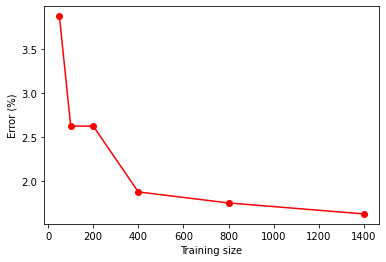
\includegraphics[width=.6\textwidth]{q4.png}
\end{figure}
The training set size of 1400 gives the best classification error.
 
\end{document}